\chapter{Results}
\label{chapter:results}
In this chapter we will discuss the results of our experiments with groups. Note that the error rate depicted in the graphs is \textit{not} the loss, but rather its square root. This is done as to represent errors on the original scale.

\section{Cyclic groups}
Cyclic groups are the simplest groups possible. They are defined as groups generated by only one element $x$. They are all isomorphic to either $(\mathbb{Z},+,-,0)$ - integers with addition - or $(\mathbb{Z}_n,+,-,0)$ - $\{0,1,2,\dots n-1\}$ with addition modulo $n$.

\subsection{$\mathbb{Z}_{10}$}

The group selected first was $\mathbb{Z}_{10}$. All elements were represented as themselves in $\mathbb{R}^1$. Since there is no element $a$ such that $a+a=1$, this was selected as the equation through which we will extend this group. Expected extension is $\mathbb{Z}_{20}$, where the embedding is $a = 1$, therefore $1_{\mathbb{Z}_{10}}\mapsto 2_{\mathbb{Z}_{20}}$. We will call this $a$ the \textit{half}.\\

The results of one experiment with training the composition, inverse and the unit are depicted in \Autoref{graph:z10_90percent}. As we can see, we can get a very good approximation of composition and the unit. The inverse lags behind a little, but that is expected because it is dependent on both of the other functions, therefore the errors in them reflect in the inverse much more. 

The inverse also appears smoother. That is because the testing set for the inverse network contains 10\% of all data, therefore here it is only one element. That means that all testing batches are the same (although that is not true for thes training batches).

One unexpected result was the fact that while in most runs the unit tended to be around $0$, sometimes it also settled around $10$. That could also be considered a right answer, although $10$ is not in the chosen representation.\\

While learning the extension, most of the time the "half" settled around $5.5$. This is of course one of two possible intuitive solutions to $a+a=1$, the other of course being $0.5$. Table \ref{table:z10_half} shows how the extension settled in several different runs. Note that the runs had different lengths, but the \textit{half} always settled so early that the length had no effect.

Table \ref{table:z10_half_generator} shows how two different runs generated $\mathbb{Z}_{20}$ using iterated (learned) composition on the "half" element.


\begin{figure}[b]
\caption{Error rate for the learning of composition, inverse and unit in $\mathbb{Z}_{10}$. Testing data percentage is 10\%}
\label{graph:z10_90percent}
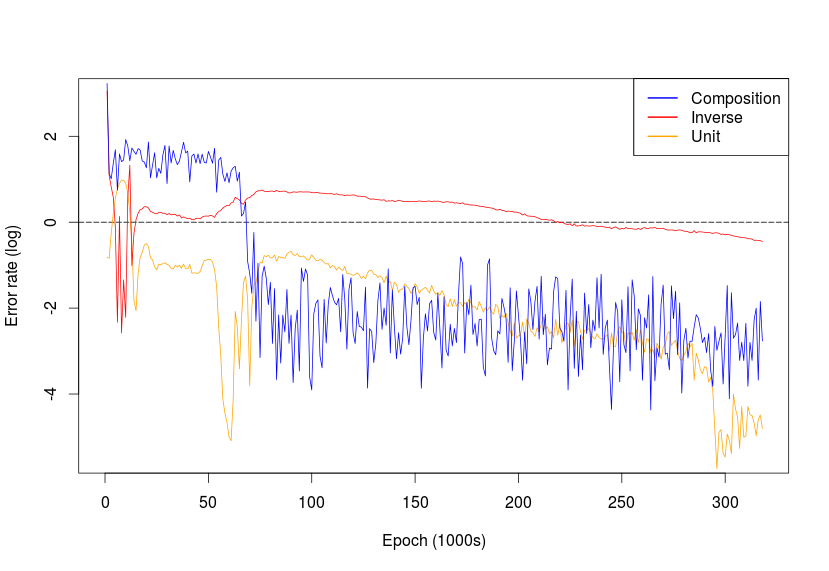
\includegraphics[width=\linewidth]{../img/z10_90percent.png}
\end{figure}
\begin{figure}[h]
\centering
\caption{Different values of "half" found during different runs. The first run (red) was very peculiar since it had over 2 700 000 epochs, but this representation settled already around epoch 300 000. It is not clear how this interacts with the rest of the elements.}
\label{table:z10_half}
\begin{tabular}{|c|c|c|c|c|c|}
\hline
\textcolor{red}{-0.9417969} & \textcolor{blue}{5.5017343} & \textcolor{blue}{5.500125} & 0.5014977 & \textcolor{blue}{5.500004} & \textcolor{blue}{5.507943}\\
\hline
\end{tabular}
\end{figure}

\begin{figure}[h]
\centering
\caption{Extension groups generated in two runs (read left to right, top to bottom). The blue elements are supposed to be in the original embedding, i.e. they should be 1...9 ascending with the last 3 elements being 0, "half", 1 respectively. In the first run we see that we have had very low success, even though the first half+half looks promising. The second run had much better success and with the exception of 9 it hit all original elements reasonably well, even those last 3.}
\label{table:z10_half_generator}
\begin{tabular}{ccccc}
\textbf{5.500004} & \textcolor{blue}{0.99998194} & 10.919293 & \textcolor{blue}{6.419118} & 1.9191066\\
 \textcolor{blue}{9.268123} & 4.7680063 & \textcolor{blue}{0.26805452} & 12.234171 & \textcolor{blue}{7.7339497}\\
3.2338893 & \textcolor{blue}{8.733828} & 4.233731 & \textcolor{blue}{1.9053116} & 9.292908 \\
\textcolor{blue}{4.792793} & 0.2928396 & \textcolor{blue}{12.189646} & 7.6894255 & \textcolor{blue}{3.1893663}\\
\textbf{8.689303} & \textcolor{blue}{4.189211}\\
 \\
\hline\\

\textbf{5.5069175} & \textcolor{blue}{0.99456155} & 6.5232387 & \textcolor{blue}{2.0135} & 7.5396843\\
\textcolor{blue}{3.032562} & 8.556266 & \textcolor{blue}{4.051762} & 3.872835 & \textcolor{blue}{5.4972463}\\
0.9848655 & \textcolor{blue}{6.5135655} & 2.0038028 & \textcolor{blue}{7.530016} & 3.022867\\
\textcolor{blue}{8.546589} & 4.04206 & \textcolor{blue}{3.9609222} & 4.6975384 & \textcolor{blue}{0.18309715}\\
\textbf{5.713754} & \textcolor{blue}{1.20193}
\end{tabular}

\end{figure}


\subsection{$\mathbb{Z}_{20}$}
The second group we experimented with was $\mathbb{Z}_{20}$. Because of its larger size, the experiments with it were longer. 

Once again, the equation by which we extend the group was $a+a=1$. The results of one experiment can be seen in \Autoref{graph:z20_90percent}. Once again, $10\%$ was excluded from the training. The trend lines are similar to $\mathbb{Z}_{10}$ (\Autoref{graph:z10_90percent}), with composition and inverse training quickly, while inverse lags behind. The inverse line is much noisier, because now the testing data has 2 elements, out of which 5 are chosen for testing (with repetition).

Values for the half in different runs can be seen in \Autoref{table:z20_half}. Once again, the algorithm usually found one of the two intuitive answers, 0.5 and 10.5. A graph showing the iterated composition of the half is depicted in \Autoref{graph:z20_half_generator}. As we see, the learned structure appears at first as very similar to the expected $\mathbb{Z}_{40}$, however we start seeing very large deviation after 40 compositions. The cause of this is unknown, but we suspect it could be caused by the network not learning the associativity axiom. Indeed, $19+1\doteq$19+(half+half) outputs correctly $0$, however (19+half)+half does not output 0.

\begin{figure}[h]
\centering
\caption{A $\mathbb{Z}_{20}$ learning run. We see that the trends we observed in $\mathbb{Z}_{10}$ continue, and it appears that extra time is not needed. However, in different runs we encountered difficulties with learning the inverse function.}
\label{graph:z20_90percent}
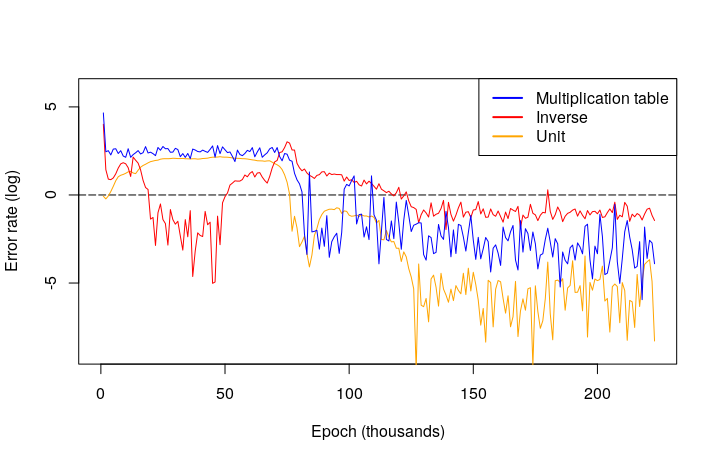
\includegraphics[width=\linewidth]{../img/z20_90percent.png}
\end{figure}

\begin{figure}[h]
\centering
\caption{Values for the half in different $\mathbb{Z}_{20}$ runs. Once again, the reason for why the red one is so different is unknown. The tendency towards 0.5 instead of 10.5 can be attributed to the fact that the initial parameters have been restricted to avoid overflow errors.}
\label{table:z20_half}
\begin{tabular}{|c|c|c|c|c|}
\hline
0.4999506 & \textcolor{red}{-6.5685954} & \textcolor{blue}{10.500707} & 0.49987993 & 0.5000777\\
\hline
0.49967808 & 0.49978873 & 0.49993014 & 0.50047106 & \textcolor{blue}{10.499506}\\
\hline
\end{tabular}
\end{figure}

\begin{figure}[h]
\centering
\caption{An example of a group generated from the "half" element. We see that there were no problems with addition of the half, except the modulus is not applied correctly.}
\label{graph:z20_half_generator}
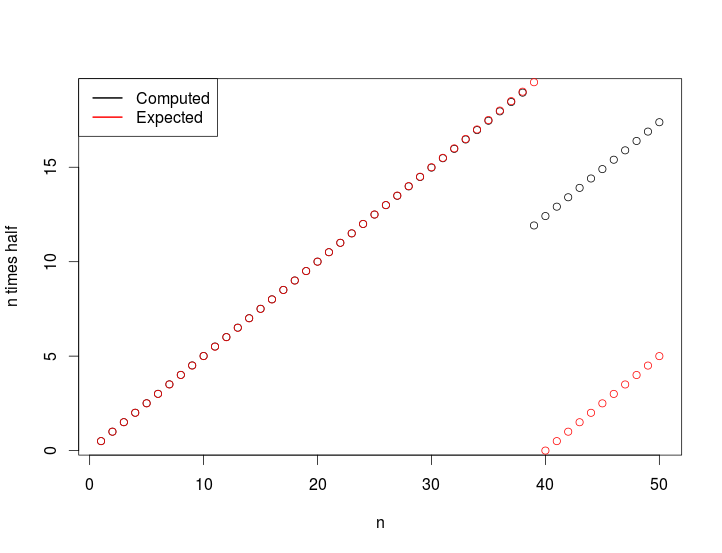
\includegraphics[width=0.8\linewidth]{../img/z20_half_plot.png}
\end{figure}

\subsection{Infinite group $\mathbb{Z}$}

The last cyclic group experiment was with the infinite group $(\mathbb{Z},+)$. The training set comprised of integers from an interval $[-10000,10000]$ in order to avoid overflow errors. Because neural network learning is already hard on such a diverse set, we opted to not exclude any data for training. 

$a+a=1$ still has no solution in this group. In contrast to the previous cases, there is only one intuitive solution and that is $\frac{1}{2}$. The group generated by this $\frac{1}{2}$ is isomorphic to the original. Unfortunately, we were unable to get to this point. The learned half was 
-1.1713637. When we tried to generate some elements of the extension, we obtained

\begin{tabular}{cccccc}
1&2&3&4&5&6\\
\hline
-1.1713637&1.0000439&2.2069557&2.8777812&3.2506382&3.4578807\\
 \\
7&8&9&10\\
\hline 
3.57307&3.637094&3.6726806&3.6924593
\end{tabular}

Indeed, the learned half+half=1, but the composition fails for larger iterations.
\begin{figure}
\caption{$\mathbb{Z}$ as an infinite group. Because of limitations of the software, we only trained on the interval $[-10000,10000]$ (hence the trained group is not really infinite). There was no testing set, but the network seemed to generalize well even outside of the training interval. Examples are computed $11000^{-1}=-11001.614$ or $15000+(-12000)=2999.9941$.}
\centering
\label{graph:z_inf}
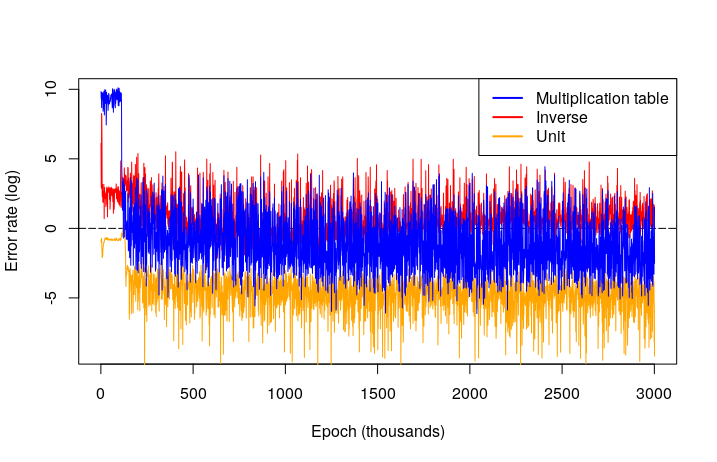
\includegraphics[width=\linewidth]{../img/z_inf.png}
\end{figure}

\section{Symmetric groups}
Symmetric groups, or permutation groups are the most complex finite groups. Indeed, a corollary from Cayley's theorem  is that every finite group is isomorphic to a symmetric group of large enough size (\cite{cayley}). This is why they have been chosen for further experiments.

Every symmetric group is generated by the set of transpositions of two elements. Each element can therefore be written as a sequence of transpositions. Although this sequence is not unique, all such sequences have the same length. For each permutation $\sigma$ we define $\text{sgn}(\sigma)=(-1)^l$ where $l$ is this number of transpositions. It also holds that $\text{sgn}(\sigma_1\circ\sigma_2)=\text{sgn}(\sigma_1)\text{sgn}(\sigma_2)$. Therefore $\text{sgn}(\sigma\circ\sigma)=1$. (proofs in \cite{Lingebra})

For this reason the equation that we sought to find the extension for is $h\circ h=(0,1)$ where $(0,1)$ denotes the transposition of elements $0$ and $1$. $\text{sgn}((0,1))=-1$, therefore we know that $h$ can not be in the original group. 

The structure of this extension is suspected to be some form of the semidirect product of $S_n\times\mathbb{Z}_2$, although the basic semidirect product appears to be insufficient.

\subsection{$S_4$ with a basic grounding}

$S_4$ is the group of permutations of 4 elements. A "na\"{i}ve" grounding of elements was chosen first. It assigns each permutation $(a,b,c,d)$\footnote{This being the full representation of the permutation.} the element $[a,b,c,d]\in\mathbb{R}^4$. The advantage of this grounding is its simplicity and shortness. The main disadvantage, however, is that the mean squared error loss function is biased. We can see this on an example where $[0,1,2,3]$ is one transposition away from both $[1,0,2,3]$ and $[3,1,2,0]$, however in the latter case the mean squared error is considerably higher. 

For the training we once again use only 90\% of the data. During the training we expectedly observe significantly higher training times, as exemplified in \Autoref{graph:s4_basic}. This is also compounded by having slightly more elements (24). We are also unable to achieve the same precision. Learning of the unit was again very precise, see table \ref{table:s4_unit_basic}.

When it comes to learning of $h$, we see even more problems than in the case of cyclic groups. Some half elements are seen in table \ref{table:s4_half_basic}. They are noticeably different from each other, something we did not observe before. The reason why these were the vectors found is unknown. 

However, as we see in table \ref{table:s4_half_basic_gen}, generating even a small subgroup results in a failure. Since $h\circ h=(0,1)$, we expect that $h^4=(h\circ h)\circ(h\circ h)=(0,1)\circ(0,1)=e$. Unfortunately, we were never able to get this equation to hold with $h\circ(h\circ(h\circ h))))$. Once again, reason for this is unknown. But because $(h\circ h)\circ (h\circ h)$ yielded reasonable results, we suspect that again the associativity is the problem.

\begin{figure}
\caption{One run of learning the $S_4$ with the basic grounding. We see that the training is expectedly much slower than in the cyclic groups.}
\label{graph:s4_basic}
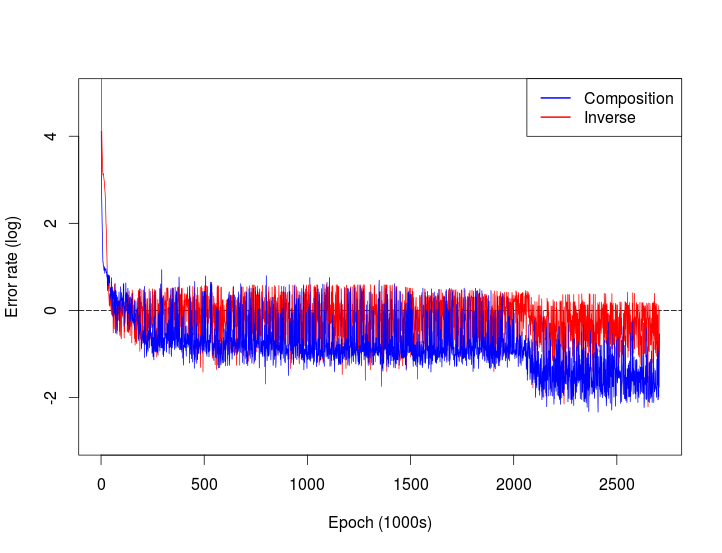
\includegraphics[width=0.9\linewidth]{../img/s4_comp+inv.png}
\end{figure}

\begin{figure}
\center
\caption{Units learned in $S_4$ with basic grounding. The expected output was $[0,1,2,3]$. As we see, they are very precise.}
\label{table:s4_unit_basic}
\begin{tabular}{l|cccc}
1.) &0.03967234 & 1.0745986 & 1.957876 & 2.9761093\\
\hline
2.) &0.00685234 & 1.0557759 & 2.1151063 & 3.2438033\\
\hline
3.) &0.01609807 & 0.9784863 & 2.011951 & 3.0008512\\
\end{tabular}
\end{figure}

\begin{figure}
\center
\caption{$h$-s found in several runs. As expected, they do not look like anything.}
\label{table:s4_half_basic}
\begin{tabular}{l|cccc}
1.)&-0.9288303 & 1.8216157 & 0.17884427 & 2.0224957\\
\hline
2.)&1.2200519 & 0.5469334 & 3.7773933 & -0.22675751\\
 \hline
3.)&2.9790108 & 2.5041845 & 1.9638568 & -1.186425\\
\end{tabular}
\end{figure}

\begin{figure}
\center
\caption{$h$ composed with itself several times. $h^2$ and $h^6$ should both be $[1,0,2,3]$. $h^4$ should be $[0,1,2,3]$.}
\label{table:s4_half_basic_gen}
\begin{tabular}{c|cccc}
$h$   & 2.9790108 & 2.5041845 & 1.9638568 & -1.186425\\
$h^2$ & 1.0137038 & 0.6440371 & 1.960084 & 3.0298772\\
$h^3$ & 1.899735 & 0.6546894 & 2.3109381 & 2.1213117\\
$h^4$ & 1.4959755 & 0.52787334 & 2.564281 & 2.4759564\\
$h^5$ & 1.3819728 & 0.7297171 & 2.8694618 & 2.1578472\\
$h^6$ & 1.1029358 & 0.97653824 & 3.1764572 & 1.9179444\\

\end{tabular}
\end{figure}

\subsection{$S_4$ with matrix grounding}
To fix the problem with the bias of the loss function we add the "one-of-n" representation. This representation is used for elements that are equally different from each other. This representation attaches to each of the $n$ elements a vector from the canonical basis of $\mathbb{R}^n$. If we take the basic representation of $S_4$ and change every element to its one-of-n representation, we get a vector in $\mathbb{R}^{16}$ that has exactly four ones and the rest are zeroes. For example 
$$(1,2,0,3)\rightarrow \left((0,1,0,0),(0,0,1,0),(1,0,0,0),(0,0,0,1)\right)$$

This erases the loss function bias, because now the mean squared difference between any two permutations depends only on the number of elements switched. One-to-n representation can also be seen as the matrix representation. Indeed, $(1,2,0,3)$ can be represented as
$$
\left(
\begin{matrix}
0 & 1 & 0 & 0\\
0 & 0 & 1 & 0\\
1 & 0 & 0 & 0\\
0 & 0 & 0 & 1
\end{matrix}
\right)
\left(
\begin{matrix}
a\\
b\\
c\\
d
\end{matrix}
\right)
=
\left(
\begin{matrix}
b\\
c\\
a\\
d
\end{matrix}
\right).
$$

A proof of this is an easy exercise in linear algebra. \\

This new grounding, however, brought several new problems. For example $3/4$-ths of the expected output are zeroes. This created a problem early on in the experimentation with the network only outputting a zero vector on any input. That is the reason why leaky ReLU had been used as an activation function as opposed to standard ReLU. This change solved this problem, since they avoid the "neuron death" - a situation where input to ReLU is so negative that it always outputs 0 and thus has no gradient.

Another problem was the size of the vectors relative to the number of elements, e.g. $S_3$ has only 6 elements but this representation has size 9. However, since the size of the group $S_n$ grows exponentially while the matrix representation only quadraticaly, for large enough $n$ the benefits of a less biased loss function outweigh the costs. Unfortunately, because of the amount of computation power needed to get to this point we were not able to verify this hypothesis.\\

As we can see in \Autoref{graph:s4_matrix}, this representation is still  efficient for composition, but the inverse is clearly wrong. Furthermore, as we see in table \ref{table:s4_matrix_unit}, the unit was usually significantly different from what was expected. This is the place where a penalty for straying away from an element could help significantly, as this problem most likely emerged as a consequence of the increase in dimension.

These two factors lead to the consequence that the inverse is not able to output elements of the grounding. If it did, composition would also output $a^{-1}a$ in grounding, but the learned $e$ is not in it.\\

The extension element $h$ is shown in table \ref{table:s4_matrix_half} along with parts of the generated subgroup. In the same vein as before, $h\circ h$ shows promise, but $h^4$ breaks down.

\begin{figure}
\center
\caption{$S_4$ with matrix grounding. The composition is very successful, but the inverse is not.}
\label{graph:s4_matrix}
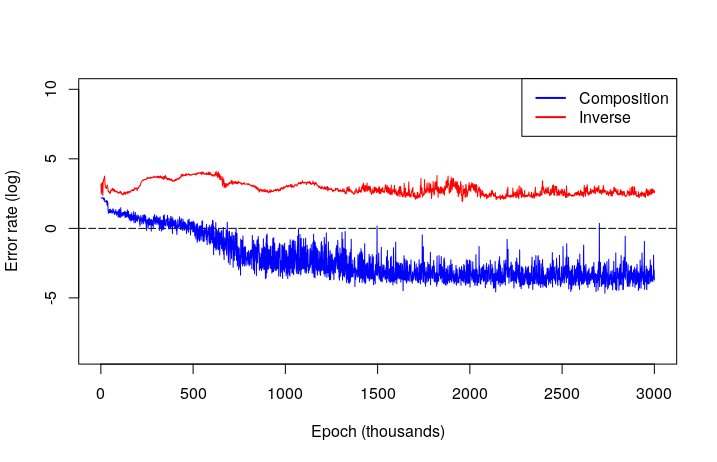
\includegraphics[width=\linewidth]{../img/s4_matrix.png}
\end{figure}

\begin{figure}
\center
\caption{Units found in $S_4$ with matrix representation. An identity matrix was expected. Places where 1 was expected are blue, black ones are for 0.}
\label{table:s4_matrix_unit}
\begin{tabular}{cccc}
\textcolor{blue}{0.9291287} & 0.39432997 & -0.09073094 & -0.00462165\\
-0.49930313 & \textcolor{blue}{2.5813785} & -1.0001388 & -0.51179993\\
0.38528794 & 0.32126167 & \textcolor{blue}{1.4879085} & -0.3122037\\
0.16110185 & -0.10436057 & -0.3780875 & \textcolor{blue}{1.356762}\\
 \\
\hline
\\
 \textcolor{blue}{0.36581007} & 0.11518399 & -0.29025748  & 0.7275856\\
0.38638538 & \textcolor{blue}{0.95944846} & -0.47597495 & -0.14604506\\
0.203323 & -0.15147878 & \textcolor{blue}{0.65808797} & -0.03862157\\
0.4341608 & -0.57306635 & -0.15940993 & \textcolor{blue}{1.5463064}
\end{tabular}
\end{figure}

\begin{figure}
\center
\caption{An extension attempt for $S_4$ with matrix representation. The blue numbers are expected to be $1$ and black ones $0$. As we see, $h^2$ is pretty much exactly what we wanted, but $h^4$ breaks down.}
\label{table:s4_matrix_half}
\begin{tabular}{lcccc}

$h$&-0.44275028 & 0.45813385 & 0.84849375 & -0.4929848\\
 &0.29338264 & 0.25557452 & 0.701611 & -0.33617198\\
 &0.5497755 & 0.75910103 & -0.16280994 & -0.17575327\\
 &0.20515643 & 0.25966993 & 0.10358979 & 1.0272595\\
 
 \hline
 
$h\circ h$&0.0016880417 & \textcolor{blue}{0.99703968} & -0.0002135747 & -0.0009868203\\
 &\textcolor{blue}{0.99901026} & -0.0018832732 & -0.0010174632 & 0.0011361403\\
 &-0.0027710588 & -0.0013556076 & \textcolor{blue}{1.0073379} & -0.001112761\\
 &-0.0005431428 & 0.0049326816 & -0.0010595275 & \textcolor{blue}{1.00323}\\
 
 \hline
 
 $h^4$&\textcolor{blue}{0.72058374} & 0.17218184	& 0.04241377 & 0.04261543\\
&0.4558762 & \textcolor{blue}{-0.00405501}	& 0.55539876 & 0.00293861\\
&-0.02832983 & 0.10163078 & \textcolor{blue}{0.4973646} & 0.4502491\\
&-0.02180864 & 0.6911213	& -0.02542126 &	\textcolor{blue}{0.4643306}

\end{tabular}

\end{figure}